\documentclass[english,a4paper,11pt,oneside,onecolumn]{book}

\usepackage{pst-all}
\usepackage{pgfplotstable}
\usepackage{url}
\usepackage{braket}
\usepackage{tikz}
\usepackage{mathtools}
\usetikzlibrary{arrows.meta}
\usepackage[utf8]{inputenc}
\setlength{\topmargin}{-1cm}
\setlength{\headsep}{.5cm}
%\setlength{\footskip}{1.0cm}
\setlength{\textheight}{24.7cm}
\setlength{\textwidth}{17cm}
\setlength{\evensidemargin}{-.5cm}
\setlength{\oddsidemargin}{-.5cm}
\usepackage{lastpage}
\usepackage{babel}
\usepackage{slantsc}
\usepackage{array}
\usepackage{csquotes}
\usepackage{listings}
\lstset{
  numbers=left,
  stepnumber=1,    
  firstnumber=1,
  numberfirstline=true,
  xleftmargin=1cm
}
\usepackage{minitoc}
\usepackage{float}
\usepackage{fancybox}
\usepackage{amsmath}
\newcommand{\EE}{\mathrm{I\!E\!}}
\newcommand{\bmat}[1]{\mbox{\boldmath $ #1 $}}
\usepackage{fancyheadings}
\usepackage{fancyhdr}
\usepackage{subcaption}
\usepackage{shadethm}
\usepackage{ifpdf}
\usepackage{amsthm}
\usepackage{lastpage}
\usepackage{makecell}
\usepackage[ruled,vlined]{algorithm2e}
%% for inserting programming code
\usepackage{minted}

%%%%%%%%%%%%%%%

\fancypagestyle{plain}{}

\pagestyle{fancy}
\lhead{\copyright Jayprakash Asolkar}
%\chead{\thepage}
\chead{\today}
\lfoot{School of Computer Science \& Statistics}
\rfoot{Trinity College Dublin, Ireland}
\cfoot{}
%%%%%%%%%%%%%%%

                

\ifpdf                                                                                           
 \pdfcompresslevel=9

\usepackage{color}


\newcommand{\red}[1]{{\color{red} #1}}
\newcommand{\solution}[1]{{\color{red} #1}}

\pdfinfo{
/Title ()
/Author ()
/Date (2016)
/Subject ()
/Keywords ()
	}
 \usepackage{graphicx}
\graphicspath{{}}
\DeclareGraphicsExtensions{.jpg,.tif,.pdf,.mps,.png}
\else                                                                                            
  \usepackage{graphicx}           
\graphicspath{{}}
\DeclareGraphicsExtensions{.eps}                                                               
\fi                        

\renewcommand{\baselinestretch}{1.5}

\usepackage{fourier}

%\usepackage[scaled]{uarial} # not available anymore
\usepackage{tgheros}
\renewcommand*\familydefault{\sfdefault} 
\usepackage[T1]{fontenc}
%preamble
\usepackage[nottoc]{tocbibind}
\usepackage[pdftex]{hyperref}                  
\hypersetup{backref,bookmarks=true,pdfpagemode=Fullscreen,linkcolor=black,colorlinks=true,urlcolor=black,citecolor=blue}

%%%%%%%%%%%%%%%%%%%%%%%%%%%%%%%%%%%%%%%%

\begin{document}
\renewcommand{\footrulewidth}{1pt}

\begin{titlepage}
	\centering
	

\includegraphics[width=.8\linewidth]{Images/trinity-common-use.jpg}\par\vspace{2cm}
% * <dahyotr@tcd.ie> 2018-02-02T15:45:10.514Z:
%
% ^.
	\vspace{2cm}
	{\huge\bfseries Data Classification using Microsoft Quantum Machine Learning Library\par}
	\vspace{1cm}
	{\scshape \par}
	\vspace{2cm}
	{\Large by Jayprakash Asolkar \par}
	{\Large Supervisor: Prof. Rozenn Dahyot \par}
 \vspace{1cm}
{\scshape 
A Dissertation submitted to the University of Dublin,\\
in partial fulfilment of the requirements for the degree of\\
Master of Science in Computer Science (Intelligent Systems),\\
School of Computer Science \& Statistics\\ 
Trinity College Dublin, Ireland\\
}
\end{titlepage}

\clearpage

\frontmatter
\pagenumbering{Roman}
\rhead{Page \thepage}
%%%%%%%%%%%%%%%%%%%%%%%%%%%%%%%%%%%%%%%%%%%%%%%%%%%%%%%%%%%%
\chapter*{Declaration}

I declare that this thesis has not been submitted as an exercise for a degree at this or
any other university and it is entirely my own work.


\vspace{3cm}
\begin{flushright}

\begin{tabular}{l}
% signature\\
\hline
\textbf{\textsf{\large Jayprakash Asolkar}}\\
\end{tabular}

\vspace{0.5cm}

\today
\end{flushright}



%%%%%%%%%%%%%%%%%%%%%%%%%%%%%%%%%%%%%%%%%%%%%%%%%%%%%%%%%%%%
\chapter*{Permission to Lend and/or Copy}

\noindent I agree to deposit this thesis in the University$\textquotesingle$s open access institutional repository or
allow the library to do so on my behalf, subject to Irish Copyright Legislation and
Trinity College Library conditions of use and acknowledgement. I agree that Trinity College Library may lend or copy this thesis upon request.

\vspace{3cm}
\begin{flushright}

\begin{tabular}{l}
% signature\\
\hline
\textbf{\textsf{\large Jayprakash Asolkar}}\\
\end{tabular}

\vspace{0.5cm}

\today
\end{flushright}

\chapter{Acknowledgments}
Firstly, I would like to thank my supervisor Prof. Rozenn Dahyot for suggesting this interesting field of research and providing immensely useful suggestions and continuous support throughout the entire process. 

Given the challenging times, this research would not have been possible without the much needed help from the online community of quantum researchers, developers and YouTube educators. I would like to thank them for their efforts in making the field of quantum computing easier to understand.

Lastly, I would like to thank my family who gave me the strength for completing my studies without any worries. 

\vspace{3cm}
\begin{flushright}

\begin{tabular}{l}
% signature\\
\hline
\textbf{\textsf{\large Jayprakash Asolkar}}\\
\end{tabular}

\vspace{0.5cm}

\today
\end{flushright}

\chapter{Abstract}
Quantum computers are slowly becoming a reality and establishing themselves as a useful piece of technology for solving a subset of real world problems which current classical computers are inefficient with. Quantum Machine Learning, a relatively new field of study, brings both the disciplines of quantum computing and machine learning  together. Although, various quantum algorithms have been theorized from long time, practical implementations of these algorithms are made possible not very long ago. Many new quantum development frameworks have recently been launched by multiple organizations to enable quantum developers and researchers to test quantum algorithms on real quantum hardware. This research documents the basics of quantum computing and information processing. Furthermore, it makes use of the machine learning library defined in Microsoft's Quantum Development Kit to classify images of hand-written digits. It presents a comparative study of a hybrid classical-quantum data classification algorithm and few of the popularly known classical machine learning algorithms.

\tableofcontents

\listoffigures

\listoftables

\mainmatter
\rhead{Page \thepage \hspace{1pt} of \pageref{LastPage}}
%%%%%%%%%%%%%%%%%%%%%%%%%%%%%%%%%%%%%%%%%%%%%%%%%%%%%%%%%%%%
%

\chapter{Introduction} 
In the recent years, Quantum Computing has attracted attention from multiple renowned researchers and computer scientists all over the globe. The credit to this growing interest in the quantum computing field can be attributed to the immense potential of this new computing paradigm to improve existing technology. Although, the current quantum technology is in very early stages of its development, the recent advancements and research results are promising for the future growth \cite{castelvecchi_2017_quantum}. 

Areas of current quantum research span across both the hardware and software realms. Exciting work is in progress to improve reliability, scalability and performance of the quantum systems. A race to build the best quantum hardware that would enable reliable real-world software application development is underway. Multiple technological companies such as Microsoft, Honeywell, 1Qubit and D-Wave are investing in quantum hardware technology based on Topological Qubits, Super-Conducting Qubits, Trapped Ions etc. All of these technologies have their own advantages and disadvantages \cite{ladd_2010_quantum}. However, exploration of various techniques to get rid of the limitations has led to many workable quantum computers \cite{castelvecchi_2017_quantum} which can be accessed via publicly available cloud resources.

Quantum algorithm development during early nineties has been major fuelling factor for the interest in the Quantum Computing field among research fraternity. Many of these algorithms are theoretically superior to best known classical algorithms. Quantum software stack is being developed with various approaches to complement the available hardware technology. A significant work is required in this field to identify suitable application areas, development of new quantum algorithms and improvement of scalability and reliability of the developed solution.

Quantum machine learning \cite{biamonte_2017_quantum} is a sub-domain of Quantum software development and has recently gained pace in terms of novel solutions. Classical machine learning technology has become better over the last few years with the advent of Neural Networks and continued research in other methodologies. However, this technology is quickly reaching a plateau in terms of new improvements and the limits of classical computation power. Quantum machine learning (QML) is trying to provide solutions to the challenges faced by classical machine learning techniques. 

This dissertation explores data classification as an application of QML and evaluates current state of the art methods. The research is based on Microsoft's application development framework for quantum computers. It makes use of the existing machine learning library to achieve the objectives. Next section discusses the motivation and aims of this research.

\section{Motivation}
\label{sec:resMotiv}

\subsection{Classical Limitations}
Classical machine learning solutions are resource intensive both in terms of required data for training as well as hardware capabilities required to process this huge amount of data. Accuracy and efficiency of classical ML algorithms depend on large amount of training data \cite{voss_2016_why}. Increase of training samples requires exponential growth of processing power and storage.

\subsection{Quantum Promises}
Quantum Computation promises to provide exponential speedups \cite{biamonte_2017_quantum, nielsen_2019_quantum, castelvecchi_2017_quantum}. Quantum Information Processing techniques can inherently compress classical data. Few of the existing quantum algorithms are theoretically superior to best known classical counterparts in terms of execution speed. Quantum Computing is naturally suitable for problems in the field of machine learning, chemistry etc.
  
\subsection{Availability of Quantum Development Frameworks}
Although, multiple software development frameworks have recently been developed \cite{cjgronlund_microsoft, asfaw_2020_learn} by various companies, there is a lack of practical implementations of available quantum algorithms over real world data sets. These frameworks give an opportunity for experimental verification of Quantum Superiority with the help of Quantum Simulators and Hardware.

\section{Research Question}
\label{sec:resQ}

\begin{displayquote}
\emph{Developing a hybrid Quantum Machine Learning (QML) application to perform binary classification of MNIST images using Microsoft Quantum Development Kit to help my reader understand the process of near term quantum application development.}
\end{displayquote}

The hybrid solution in the research question specifies that the quantum application makes use of both the classical and quantum hardware to perform desired tasks. Due to the time constraints this work focuses only on binary classification of the given dataset. This dissertation hopes to provide a guidance for future application development and research in the quantum computation field.

\section{Research Objectives}
\label{sec:resObj}
Below mentioned objectives are necessary to answer the research question of this dissertation.
\begin{itemize}
  \item Learning about Quantum Computation and Quantum Information Processing. This is helpful to understand the basic building blocks of a quantum computer. Also, it serves the readers to gain important knowledge about quantum computation, who are beginning their journey in the similar field of research.
  \item Understanding the State of the Art of Quantum Machine Learning for data classification. A lot of research work is initiated very recently in the QML field of study.
  \item Evaluation of Data Classification library in Microsoft Quantum Development Kit on real world dataset. This research aims to perform multiple experiments to assess the capabilities of the new data classification framework in Microsoft QDK.
  \item Identifying  useful resources and current challenges for real world application development using Microsoft QDK. This dissertation tries to be a quick reference for starting future research in quantum application development which involves both quantum and classical hardware.
\end{itemize}

\section{Dissertation Structure}
\label{sec:dissStruc}
The dissertation is structured as specified below.

\begin{itemize}
  \item Chapter 2 provides information about basics of quantum computing. This is important for building an intuition of how a quantum computer works. Also this chapter gives an overview of multiple quantum algorithms.
  \item Chapter 3 discusses about the open source quantum application development framework developed by Microsoft. It further lists down the reasons behind selecting this framework for the implementation of this dissertation. Basics of Q\# programming are discussed in this chapter
  \item Chapter 4 presents the design of Circuit Cetric Quantum Classifier. It details the interactions between various components involved in the data classification process.
  \item Chapter 5 provides details about the implementation strategy followed to achieve the objectives of the dissertation.
  \item Chapter 6 shows the results obtained by the execution of various iterations of quantum experiments. It also displays a comparison between results obtained from quantum and classical programs.
  \item A detailed discussion about the results obtained and evaluation of the followed strategy is presented in the chapter 7.
  \item Chapter 8 concludes the research by discussing contributions of the dissertation along with suggestions to be followed for future work in the same domain.
\end{itemize}

%%%%%%%%%
\chapter{Background Research}
\label{sec:soa}

The development of Quantum Mechanics over the last century has paved the way for the new paradigm of computation. Paul Benioff with his research on Quantum Information and Quantum mechanical model of Turing Machines pioneered the field of Quantum Computing. Quantum computation is based on the postulates of quantum mechanics which define the way quantum systems behave. In the last couple of decades, many theoretical quantum algorithms have been developed which suggest a possible superiority of quantum computers over their classical counterparts. This section discusses, in brief, the basics of quantum computing required to build more complex algorithms which can help to solve some of the challenging problems faced by classical computers. It is important to have a solid understanding of basic linear algebra \cite{a3blue1brown_2016_vectors} to understand the maths behind quantum computation. Furthermore, this section gives an overview of state of the art applications of quantum computing across various domains.

\section{Quantum Bit}
\label{sec:qubit}

The most basic unit of computation for classical computers is a bit (binary digit) which is used to store and process information. Quantum computers make use of a similar unit of information called Quantum Bit or Qubit. Unlike the classical bit which can represent either a zero state or one state at any given time, a qubit can simultaneously be in a superposition state of both $\ket{0}$ and $\ket{1}$ state \cite{nielsen_2019_quantum}. More precisely, the state of a single qubit is a unit vector in a 2-dimensional complex vector space called Hilbert Space. The special states $\ket{0}$ and $\ket{1}$, of the qubit vector are called the orthonormal basis of the Hilbert space. Any arbitrary state \(\ket{\psi}\) of the qubit can be defined as a linear combination of the basis vectors.
\begin{equation}\label{eq:1}
    \ket{\psi} = \alpha\ket{0} + \beta\ket{1} \hspace{25pt}where\hspace{10pt} \braket{\psi|\psi} = |\psi|^2 = 1
\end{equation}

In the equation \ref{eq:1}, \(\alpha\) and \(\beta\) are complex numbers and \(|\alpha|^2\), \(|\beta|^2\) are the probabilities of measuring the qubit in $\ket{0}$ or $\ket{1}$ basis states respectively. The matrix representation of the arbitrary qubit state \(\ket{\psi}\) and basis states \(\ket{0}\), \(\ket{1}\) is given by equation \ref{eq:2}. On an ideal quantum computer, measurement of a qubit in $\ket{0}$ basis state yields the binary digit 0, hundred percent of the times. Similarly there is 100\% probability of a qubit in $\ket{1}$ state resulting in the measurement of binary digit 1. 
\begin{equation}\label{eq:2}
\ket{\psi} = 
\begin{bmatrix}
\alpha\\
\beta
\end{bmatrix}\hspace{25pt}
\ket{0} = 
\begin{bmatrix}
1\\
0
\end{bmatrix}\hspace{25pt}
\ket{1} = 
\begin{bmatrix}
0\\
1
\end{bmatrix}
\end{equation}
The pure state of a qubit can also be thought as a point residing on the surface of the Bloch Sphere. Figure \ref{fig:bloch1} shows the Bloch sphere representation of the qubit state vector. The $\theta$ , $\phi$ are

\begin{figure}[H]
\centering
 \begin{tikzpicture}[line cap=round, line join=round, >=Triangle]
  \clip(-2.19,-2.49) rectangle (2.66,2.58);
  \draw [shift={(0,0)}, lightgray, fill, fill opacity=0.1] (0,0) -- (56.7:0.4) arc (56.7:90.:0.4) -- cycle;
  \draw [shift={(0,0)}, lightgray, fill, fill opacity=0.1] (0,0) -- (-135.7:0.4) arc (-135.7:-33.2:0.4) -- cycle;
  \draw(0,0) circle (2cm);
  \draw [rotate around={0.:(0.,0.)},dash pattern=on 3pt off 3pt] (0,0) ellipse (2cm and 0.9cm);
  \draw (0,0)-- (0.70,1.07);
  \draw [->] (0,0) -- (0,2);
  \draw [->] (0,0) -- (-0.81,-0.79);
  \draw [->] (0,0) -- (2,0);
  \draw [dotted] (0.7,1)-- (0.7,-0.46);
  \draw [dotted] (0,0)-- (0.7,-0.46);
  \draw (-0.08,-0.3) node[anchor=north west] {$\varphi$};
  \draw (0.01,0.9) node[anchor=north west] {$\theta$};
  \draw (-1.01,-0.72) node[anchor=north west] {$\mathbf {\hat{x}}$};
  \draw (2.07,0.3) node[anchor=north west] {$\mathbf {\hat{y}}$};
  \draw (-0.5,2.6) node[anchor=north west] {$\mathbf {\hat{z}=|0\rangle}$};
  \draw (-0.4,-2) node[anchor=north west] {$-\mathbf {\hat{z}=|1\rangle}$};
  \draw (0.4,1.65) node[anchor=north west] {$|\psi\rangle$};
  \scriptsize
  \draw [fill] (0,0) circle (1.5pt);
  \draw [fill] (0.7,1.1) circle (0.5pt);
 \end{tikzpicture}
\caption{Bloch Sphere representation of single qubit} \label{fig:bloch1}
\end{figure}

North and south poles of the sphere represent $\ket{0}$, $\ket{1}$ states respectively. As shown in equation \ref{eq:3} \cite{nielsen_2019_quantum}, by ignoring the global phase, angles \(\theta\) and \(\varphi\) can be used to define any arbitrary state of a qubit. 

\begin{equation}\label{eq:3}
    \ket{\psi} = cos\hspace{2}\dfrac{\theta}{2}\hspace{2}\ket{0} + e^i^\varphi \hspace{2}sin\hspace{2}\dfrac{\theta}{2}\hspace{2}\ket{1}
\end{equation}

Real quantum computers make use of atoms, trapped ions, electrons, photons to realize quantum bits \cite{ladd_2010_quantum}. Physically $\ket{0}$ and $\ket{1}$ states may correspond to polarization of a photon or the alignment of nuclear spins.

\section{Multiple Qubits and Entanglement}
\label{sec:multiQubit}
A single qubit alone is not sufficient to perform quantum computation. The power of quantum computers lies in the use of registers of qubits and their co-related states. Using n qubits in superposition state of $\ket{0}$ and $\ket{1}$, for eg. \(\dfrac{\ket{0} + \ket{1}}{\sqrt{2}}\), we can represent \(2^n\) states simultaneously in a multi-qubit system. However, it should be noted that measurement of the state of a qubit collapses the state to one of the basis states and destroys the quantum information. Hence, at any given time, only a single state can be retrieved through measurement of a quantum system. This remains a challenge in developing efficient quantum algorithms.

A multiple qubit system with n qubits has \(2^n\) computational basis states. These basis states of a multi-qubit system can be obtained by using tensor product of the basis states of individual qubits (For eg. \(\ket{00} = \ket{0}\otimes\ket{0}\)). Equation \ref{eq:4} represents an arbitrary state $\ket{\psi}$ in 2-qubit system. 

\begin{equation}\label{eq:4}
    \ket{\psi} = \alpha\ket{00} + \beta\ket{01} + \gamma\ket{10} + \delta\ket{11} \hspace{15} where \hspace{10} |\alpha|^2 + |\beta|^2 + |\gamma|^2 + |\delta|^2 = 1
\end{equation}

An important feature of multi-qubit quantum system is the ability to prepare entangled states of two or more qubits. The states of 2 entangled qubits affect each other even if the qubits are separated by a long distance. The entangled state \(\dfrac{\ket{00} + \ket{11}}{\sqrt{2}}\) is called the Bell state or EPR pair and is the basic ingredient of multiple quantum algorithms. The terminology entanglement of two qubits specifies that the measurement of the state of only a single qubit among the EPR pair is sufficient to predict the outcome of measurement of the second qubit with absolute certainty.

\section{Quantum Gates}
\label{sec:qGates}
For any meaningful computation, the ability to manipulate states of the qubits is essential. Various quantum gates are the means to linearly transform the state vector of a single qubit or register of multiple qubits. Quantum computers make use of lasers, magnetic fields or other technologies to physically alter the qubit state.

Similar to classical logic gates namely AND, OR, XOR etc., quantum computers make use of quantum gates which linearly change the qubit state vector. The Pauli-X gate is similar to classical NOT gate and acts on a single qubit to change the state from \(\ket{0}\) to \(\ket{1}\) and vice versa \cite{matuschak_2019_quantum}. The Pauli-X gate is represented in matrix format as shown in equation \ref{eq:5}.
\begin{equation}\label{eq:5}
X = 
\begin{bmatrix}
0 & 1\\
1 & 0
\end{bmatrix}
\end{equation}

The quantum Pauli-X gate acts linearly on the arbitrary state $\ket{\psi}$ to swap the measurement probabilities of \(\ket{0}\) and \(\ket{1}\) vectors. The equation \ref{eq:6} shows the application of the Pauli-X gate as the inner product of the gate with the state vector.
\begin{equation}\label{eq:6}
X\ket{\psi} = \alpha X \ket{0} + \beta X \ket{1} = 
\alpha
\begin{bmatrix}
0 & 1\\
1 & 0
\end{bmatrix}
\begin{bmatrix}
1\\
0
\end{bmatrix} + 
\beta
\begin{bmatrix}
0 & 1\\
1 & 0
\end{bmatrix}
\begin{bmatrix}
0\\
1
\end{bmatrix} = 
\alpha
\begin{bmatrix}
0\\
1
\end{bmatrix} + 
\beta
\begin{bmatrix}
1\\
0
\end{bmatrix} =
\alpha\ket{1} + \beta\ket{0}
\end{equation}

The Pauli-Y and Pauli-Z gates are other two gates in the Pauli set and both of these act on a single qubit. Another important single qubit gate is the Hadamard gate. The Hadamard gate creates an equal superposition of both the computational basis states. Matrix representation of Pauli-Y, Pauli-Z and Hadamard gates is given by equation \ref{eq:7}. 

\begin{equation}\label{eq:7}
Y = 
\begin{bmatrix}
0 & -i\\
i & 0
\end{bmatrix}
\hspace{25pt}
Z = 
\begin{bmatrix}
1 & 0\\
0 & -1
\end{bmatrix}
\hspace{25pt}
H = \dfrac{1}{\sqrt{2}}
\begin{bmatrix}
1 & 1\\
1 & -1
\end{bmatrix}
\end{equation}

Quantum computation also makes use of gates acting on states of multiple qubits. A 4x4 CNOT gate acts on a register of 2 qubits. One of the qubits acts as the control qubit whereas another qubit in the set is called the target qubit. Based on the state of control qubit, the CNOT gate acts on the target qubit to flip its state. If the control qubit is in the state \(\ket{0}\) then the CNOT gate does nothing to the target qubit and its state remains unchanged, whereas if the control qubit is in the state \(\ket{1}\), the CNOT gate acts as a X gate on the target qubit. The dimensions of the matrix of a multi-qubit gate acting on n qubits is \(2^n\)x\(2^n\).

\begin{equation}\label{eq:8}
U_{CNOT} = 
\begin{bmatrix}
1 & 0 & 0 & 0\\
0 & 1 & 0 & 0\\
0 & 0 & 0 & 1\\
0 & 0 & 1 & 0
\end{bmatrix}
\end{equation}

All quantum gates are unitary matrices i.e. the hermitian conjugate or adjoint of the gate matrix is also the inverse of the matrix. A hermitian conjugate is obtained by flipping the given matrix over its diagonal and changing the sign of the imaginary parts of the complex numbers. This constraint on the quantum gates makes them reversible. Hence, information about the input to the quantum gate never gets lost unlike the classical logic gates. Equation \ref{eq:9} is true for every quantum gate U and depicts that applying any gate twice on input qubit states restores the original quantum state. Also, unitary matrices maintain the normalization condition of the qubit state given by \(|\alpha|^2\) + \(|\beta|^2\) = 1.

\begin{equation}\label{eq:9}
UU^\dagger = I \hspace{25} where \hspace{5}U^\dagger = Adjoint(U)
\end{equation}

As shown in equations \ref{eq:10} and \ref{eq:11}, the reversibility of quantum gates can be verified for any of the gates discussed so far. 
\begin{equation}\label{eq:10}
HH = 
\dfrac{1}{\sqrt{2}}
\begin{bmatrix}
1 & 1\\
1 & -1
\end{bmatrix}
\hspace{10}
\dfrac{1}{\sqrt{2}}
\begin{bmatrix}
1 & 1\\
1 & -1
\end{bmatrix}
=
\begin{bmatrix}
1 & 0\\
0 & 1
\end{bmatrix}
=I
\end{equation}
\begin{equation}\label{eq:11}
HH\ket{\psi} = I \ket{\psi} = \ket{\psi}
\end{equation}

Effect of any arbitrary quantum gate on the state of a qubit can be thought of as a rotation of the state vector around different axes in the Bloch sphere \cite{nielsen_2019_quantum}. Additionally, any arbitrary transformation of the qubit state can be achieved by using combination of few basic gates.

\section{Quantum Circuits}
\label{sec:qCirc}
Quantum algorithms are depicted using the circuit model of computation. A quantum circuit comprises of register of qubits, quantum gates and measurements in classical bits. Logically, the simplest possible quantum circuit is a quantum wire which retains the state of a qubit over a period of time or a communication channel. However, this is the most difficult quantum circuit to implement physically, as the state of a qubit gets easily affected by its environment, corrupting the quantum information. 

\begin{figure}[H]
    \centering
    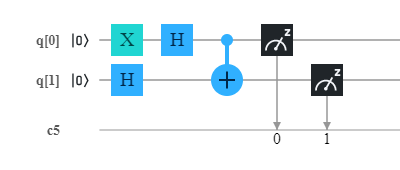
\includegraphics[scale=0.7]{Images/quantumCircuitExample.png}
    \caption{An example of quantum circuit visualized using IBMQ circuit composer \cite{asfaw_2020_learn}}
    \label{fig:qCircEx}
\end{figure}

Figure \ref{fig:qCircEx} shows the composition of a quantum circuit. Two qubits \(q_0\) and \(q_1\) of the quantum register are prepared in the \(\ket{0}\) basis state. The qubit \(q_0\) is passed through the quantum wire across the X and Hadamard gates, whereas the qubit \(q_1\) is passed through the quantum wire across the Hadamard gate. The 2-qubit CNOT gate uses \(q_0\) as the control qubit and works on the target qubit \(q_1\). Finally both the qubits are measured on the classical channel c5. After the measurement, the state of each of the qubits collapses to the computational basis state. More complex circuits can be built in similar way to realize various quantum algorithms which can utilize quantum properties such as superposition and entanglement.

\section{Quantum Computing - Hype and Promises}
\label{sec:qHype}
The Deutsch-Jozsa algorithm \cite{aradyamath_2019_quantum} was one of the first algorithms which showed that the quantum computers can be used to achieve exponential speedups using quantum parallelism over the best known classical algorithms. Shor's prime factoring algorithm \cite{shor_2019_algorithms} was a catalyst for the growing interest in quantum computing and quantum cryptography. It makes use of the efficiency of quantum fourier transform to find prime factors of given number N in polynomial time. No known classical algorithm exists that can acheive the same task polynomially even on best super computers. Grover's search algorithm \cite{grover_1996_a} provides quadratic speed improvement for searching a database with unsorted entries.
Currently available quantum computers are still in early stages of development and thus restrict the practical verification of many theoretical algorithms which claim quantum supremacy. Furthermore, these machines are prone to errors due to environmental interference and decoherence \cite{schuld_2020_circuitcentric}, which is an active area of research in the field of quantum computation. However, steady growth of number of qubits and power of quantum computers, cloud access to physical systems and arrival of various software development kits for programmers all around the world to develop and test new algorithms, are some of the encouraging factors for research in this area.
The no-cloning theorem \cite{wootters_1982_a} of quantum bits states that quantum information stored in one qubit can not be copied to another qubit without altering the state of the original qubit. This phenomenon has implications in the field of quantum cryptography and future of data security. Quantum chemistry is a major field of research as quantum computers can simulate quantum systems efficiently. Classical computers require exponentially increasing resources for simulation of such quantum information. Multiple companies have recognized the vast potential of quantum computers and are investing heavily in the field. Quantum machine learning, image processing, data analysis are few more fields that are gaining interest from scholars all around the globe.

\section{Introduction to Quantum Algorithms}
\label{sec:qAlgo}
As discussed in previous sections a quantum algorithm can be described using a quantum circuit consisting of qubits prepared in the desired state, gates acting on the state vector of the qubits and measurement operations in the computational basis states. This section discusses in brief few of the most important algorithms in quantum computation. Discussion on mathematical derivations of the algorithms is out of the scope of this dissertation. All these algorithms \cite{emma_2011_an} form the basis of many complex quantum algorithms and are essential in understanding how quantum computers can be utilized to solve problems.

\subsection{Quantum Superposition}
\label{sec:qSupPos}
Quantum Superposition \cite{nielsen_2019_quantum} is a quantum mechanical phenomena wherein a single qubit occupies multiple possible states at any given time. Although this state is not directly observable by any measurement apparatus, its applicability in quantum parallelism gives an edge to quantum computers over their classical counterparts to carry out multiple operations on the qubits at any single instance. If the computational states of measurement are \(\ket{0}\) and \(\ket{1}\), then an equal superposition of these two states can be obtained by applying the Hadamard transformation to the register of input qubits. Figure \ref{fig:qSupPos} shows the circuit to achieve the Hadamard transformation which achieves an equal superposition state of all possible states of individual qubits. If n is the number of input qubits and N=\(2^n\) are the computational basis states of the combination of the qubits, then the probability of measuring the qubits in any of the basis states is equal to \(\dfrac{1}{N}\). For the 3 qubit circuit, possible basis states are \(\ket{000}\), \(\ket{001}\), \(\ket{010}\), \(\ket{011}\), \(\ket{100}\), \(\ket{101}\), \(\ket{110}\) and \(\ket{111}\). After hadamard transform, the measurment probability of each of these states is \(\dfrac{1}{8}\). This forms the basis for the algorithm of random number generation in quantum computers.

\begin{figure}[H]
    \centering
    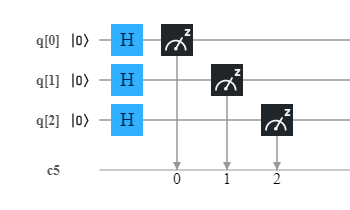
\includegraphics[scale=0.7]{Images/Quantum Superposition.png}
    \caption{Circuit to create equal superposition of the states of 3 qubits}
    \label{fig:qSupPos}
\end{figure}

\subsection{Quantum Teleportation}
\label{sec:qTele}
Quantum Teleportation makes use of quantum entanglement of qubits to communicate the information about an arbitrary state of a qubit between two parties. Consider a scenario where Alice has a qubit in the state \(\alpha\ket{0} + \beta\ket{1}\). As the knowledge about the parameters \(\alpha\) and \(\beta\) can not be obtained by classical measurement, Alice can not communicate this information directly to Bob using classical channels. However, Alice and Bob both possess a single qubit of the entangled pair \(\dfrac{\ket{00} + \ket{11}}{\sqrt{2}}\). This entangled pair can be used to send arbitrary state \(\ket{\psi}\) of a qubit from Alice to Bob.
\begin{figure}[H]
    \centering
    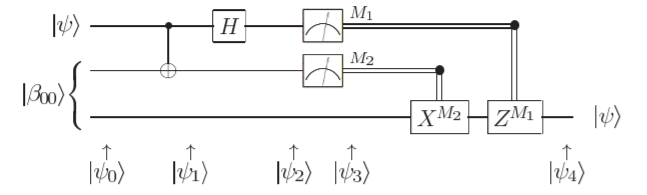
\includegraphics[scale=0.7]{Images/quantumTeleport.png}
    \caption{Circuit for Quantum Teleportation \cite{nielsen_2019_quantum}}
    \label{fig:qTelePort}
\end{figure}
\noindent In this algorithm, Alice has a qubit in arbitrary state \(\ket{\psi}=\alpha\ket{0} + \beta\ket{1}\) and one of the entangled pair of qubits, while the other qubit of the entangled pair is in the possession of Bob. Initial state of the 3 qubits together can be specified as \(\ket{\psi_0}=\dfrac{1}{\sqrt{2}}\left[\alpha\ket{0}\left(\ket{00}+\ket{11}\right)+\beta\ket{1}\left(\ket{00}+\ket{11}\right)\right]\). Alice applies a CNOT gate with the arbitrary qubit as a control qubit and entangled qubit as the target qubit. This changes the state to \(\ket{\psi_1}=\dfrac{1}{\sqrt{2}}\left[\alpha\ket{0}\left(\ket{00}+\ket{11}\right)+\beta\ket{1}\left(\ket{00}+\ket{01}\right)\right]\). The state \(\ket{\psi_2}\), after applying the Hadamard gate to the arbitrary qubit is given by equation \ref{eq:11}.
\begin{equation}\label{eq:11}
\ket{\psi_2}=\dfrac{1}{2}\left[\ket{00}\left(\alpha\ket{0}+\beta\ket{1}\right)+\ket{01}\left(\alpha\ket{1}+\beta\ket{0}\right)+\ket{10}\left(\alpha\ket{0}-\beta\ket{1}\right)+\ket{11}\left(\alpha\ket{1}-\beta\ket{0}\right)\right]
\end{equation}

Alice does the measurement of both the qubits and shares the classical measurement result with Bob. Depending on the result of Alice's measurements, Bob applies unitary transformations to his qubit to obtain the arbitrary state.

\begin{table}[!h]
\begin{center}
\begin{tabular}{|c|c|c|}
\hline
\textbf{Measurement Result} & \textbf{Bob's Qubit State} & \textbf{Transformation} \\
\hline
00 & \(\alpha\ket{0}+\beta\ket{1}\) & No Transformation Required\\
\hline
01 & \(\alpha\ket{1}+\beta\ket{0}\) & Apply Pauli-X gate \\
\hline
10 & \(\alpha\ket{0}-\beta\ket{1}\) & Apply Pauli-Z gate \\
\hline
11 & \(\alpha\ket{1}-\beta\ket{0}\) & Apply Pauli-X followed by Pauli-Z gate\\
\hline
\end{tabular}
\end{center}
\caption{Transformation on Bob's qubit for Teleportation} 
\label{tab:qTelePort}
\end{table}

This algorithm is in accordance with the no-cloning theorem and does not copy the state of Alice's qubit to Bob's qubit. The arbitrary state of Alice's qubit is destroyed due to the measurement before teleportation. This algorithm is the basis of quantum communication.

\subsection{Grover's Search Algorithm}
\label{sec:groverAlgo}
Consider a database with N entries of bit strings without any well defined structure. This database contains a bit string \(x_1\) such that f(\(x_1\))=1. For all other bit strings in the database f(x)=0. In the worst case, best known classical algorithms require to scan all the entries in the database to find \(x_1\) resulting in the complexity of O(N). Grover's search algorithm solves this problem with a quadratic speedup over the classical algorithms.\\

\begin{figure}[H]
    \centering
    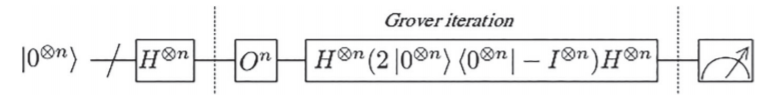
\includegraphics[scale=0.7]{Images/GroversCircuit.png}
    \caption{Grovers Algorithm - Circuit Diagram}
    \label{fig:groverCircuit}
\end{figure}

\begin{figure}[H]
    \centering
    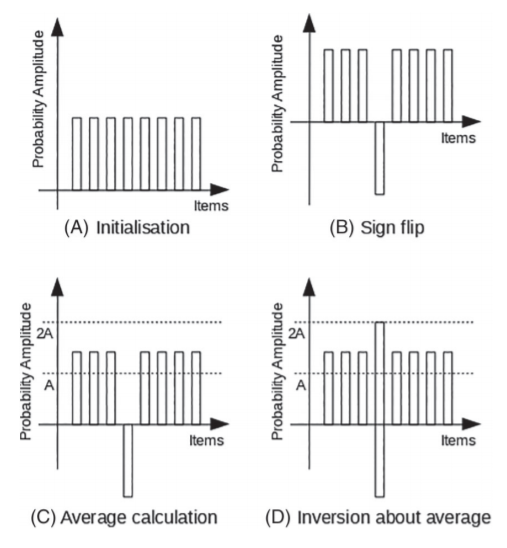
\includegraphics[scale=0.8]{Images/GroversSteps.PNG}
    \caption{Grovers Algorithm - Steps}
    \label{fig:groverSteps}
\end{figure}

Grovers algorithm works by initializing state vector in equal superposition of n=\(log_2\)N qubits using the hadamard transformation. It then applies the Grover's iteration \cite{grover_1996_a} on the register of qubits which involves phase flip of the desired state followed by state inversion about the mean as shown in figure \ref{fig:groverSteps}. Grover's iteration is repeated \(\sqrt{N}\) times to achieve the desired measurement with high probability. The circuit diagram for Grover's algorithm is shown in figure \ref{fig:groverCircuit}.

\subsection{Shor's Factoring Algorithm}
\label{sec:shorAlgo}
Shor's algorithm \cite{shor_2019_algorithms} makes use of quantum fourier transform to find prime factors of a number within polynomial time as opposed to classical algorithms which take an exponential time. This algorithm can be understood by taking a simple example of finding the prime factors of number 15. The algorithm selects a random number less than 15 which is co-prime with 15. Using the randomly selected number Shor's period finding algorithm finds the period r such that \(a^r\) mod N = 1 and \(r \neq 0\). If r is even, then there is a high probability that the greatest common divisor of either \(\left(a^\frac{r}{2} + 1\right)\) and N or \(\left(a^\frac{r}{2} - 1\right)\) and N, is a prime factor of N. If r is odd, then the algorithm repeats the steps till it finds an even r. For our example, if the randomly selected number is 7, then the period is 4 as shown in the table \ref{tab:shorPeriodFinding}. So, prime factors of 15 can be calculated by finding the GCD of \(7^2\) + 1 = 50 \& 15 which is 5 and the GCD of \(7^2\) - 1 = 48 \& 15 which is 3. The period finding part in this algorithm makes use of quantum fourier transform which takes polynomial time. 

\begin{table}[!h]
\begin{center}
\begin{tabular}{|c|c|c|}
\hline
\(7^0\) mod 15 $\equiv$ 1 mod 15\\
\hline
\(7^1\) mod 15 $\equiv$ 7 mod 15\\
\hline
\(7^2\) mod 15 $\equiv$ 4 mod 15\\
\hline
\(7^3\) mod 15 $\equiv$ 13 mod 15\\
\hline
\(7^4\) mod 15 $\equiv$ 1 mod 15\\
\hline
:\\
:\\
\hline
\end{tabular}
\end{center}
\caption{Period finding of Shor's algorithm} 
\label{tab:shorPeriodFinding}
\end{table}

\section{Designing a Quantum Algorithm}
\label{algoDesign}
While designing a quantum algorithm few constraints of the underlying quantum hardware need to be considered \cite{j_2020_quantum}. These constraints include:

\begin{itemize}
    \item Available gate set which the algorithm designer can use to program the circuit
    \item Available physical gate set
    \item Available connections between qubits
    \item Errors in the quantum hardware
\end{itemize}

For eg. IBM's QISKIT provides a gate set which has following (equation: \ref{eq:18}) logical gates available for programming a circuit \cite{j_2020_quantum}.

\begin{equation}\label{eq:18}
    \{I, X, Y, Z, H, S, S\dagger, T, T\dagger, U_1(\lambda), U_2(\lambda, \phi), U_3(\lambda, \phi, \theta), CNOT\}
\end{equation}

However, actual underlying hardware only implements ${U_1(\lambda), R_X(\pi/2), CNOT}$ gates. All other logical gates are composed of combination of these physical gates. Additionally, IBM's ibmqx4 quantum computer has 5 qubits with only 6 pairs of connected qubits. For a fully connected 5 qubit system there should be total 20 pairs of connected qubits. Quantum gate fidelity is one of the source of errors as user specified logical gate may not be accurately transferable to a set of physical gates. Also, physical quantum systems over time lose the quantum state and behave like classical states due to decoherence which gives rise to errors. All these constraints of the physical quantum hardware need to be taken into account while designing any quantum algorithm. Depth of a quantum circuit, Gate fidelity, various sources of noise in the quantum hardware can affect the accuracy of the results of an algorithm on a physical quantum system.

\section{Quantum Data Classification}
\label{sec:qml}
Classical machine learning technology has been developed over the last few decades and has provided ingenious solutions to various computational problems. Applications utilizing machine learning techniques span across fields like healthcare, industrial automation, image processing, automobiles etc. Recent progress in neural networks has improved the accuracy of these applications even further. However, efficiency and accuracy of most of the machine learning algorithms depends on big data analysis and this is a challenge for classical computers due to the huge growth of required data \cite{voss_2016_why}.\par
Recent work in the field of Quantum Machine Learning claims to have achieved significant speed improvements over best available classical algorithms \cite{schuld_2020_circuitcentric}. Quantum ML algorithms can be broadly classified into 3 categories \cite{zhang_2020_recent}. The first category contains classical ML algorithms converted to be executed on quantum computers. Second category of QML algorithms are called quantum inspired ML algorithms and take inspiration from quantum principles to improve performance. Hybrid classical-quantum machine learning algorithms fall into third category and make use of classical computers along with quantum subroutines. Many of the Quantum ML techniques such as Quantum Support Vector Machines and Quantum Principle Component Analysis \cite{lloyd_2014_quantum} are based on the HHL quantum algorithm for solving linear equations. Conversely, quantum K-Means clustering algorithm makes use of Grover's search algorithm along with Phase estimation and Swap-Test.\par
Data Classification is one of the most basic machine learning application. Recently many supervised and unsupervised learning algorithms are implemented in quantum computers for classifying input data vectors. For these methods to work, classical data which is represented in bit strings needs to be encoded in the states of qubits. Basic encoding of classical data does 1:1 mapping of bit information into qubits. In this method, a bit string 1111 will be represented using qubit state vector as \(\ket{1111}\). Although this is a simple method of data representation, it does not provide any quantum advantage. Another approach called Amplitude encoding \cite{schuld_2020_circuitcentric} stores the classical information in the amplitudes $\alpha$ and $\beta$ of the state vector $\ket{\psi} = \alpha\ket{0} + \beta\ket{1}$. This method is used in many QML algorithms and requires the classical data vector to be normalized before encoding.\par
Due to growing interest in extracting the benefits of possible quantum advantage, multiple researchers and organizations have introduced development kits for programming quantum computers \cite{asfaw_2020_learn, cjgronlund_microsoft}. Various quantum algorithms can be executed on quantum simulators as well as real quantum computers via cloud access. IBM's QISKIT \cite{asfaw_2020_learn}, Google Cirq, Microsoft's Quantum Development Kit (QDK), XANADU's PennyLane are few of the available frameworks for quantum development. Few of these frameworks also have implementations for quantum machine learning algorithms. This dissertation presents a review and evaluation of machine learning library in Microsoft's QDK framework. This library can be used for the supervised QML tasks of data classification.\par
The machine learning library in QDK uses hybrid QML approach incorporating both classical and quantum computers \cite{schuld_2020_circuitcentric}. It uses a shallow circuit utilizing limited number of qubits and quantum gates to reduce errors on currently available noisy quantum computers and claims to achieve comparable results with current state of the art methods. Amplitude encoding is used to represent classical data into the state of the qubits. Quantum entanglement captures the correlation between different qubits to predict classes of input data. The library is open sourced by Microsoft and is available for review. Next sections discuss the working of various parts of the classification algorithm along with its evaluation on different datasets.\par 

%%%%%%%%
\chapter{Microsoft Quantum Development Kit}
\label{sec:MSFTQDK}
Microsoft is one among many organizations which are actively investing in the future of Quantum technology. The technology stack \cite{cjgronlund_microsoft} as shown in figure \ref{fig:msQStack}, involves building quantum hardware or collaborating with hardware providers, developing software development frameworks along with simulators and building applications on top of the development kits for solving multiple problem areas. Microsoft plans to make these resources available commercially and for research using hybrid cloud computing. Microsoft has partnered with multiple quantum hardware and software providers for building the ecosystem. This chapter discusses the motivation behind choosing Microsoft QDK for the research. Also, it provides an overview of the Q\# programming language and other resources provided by the quantum development kit.

\begin{figure}[H]
    \centering
    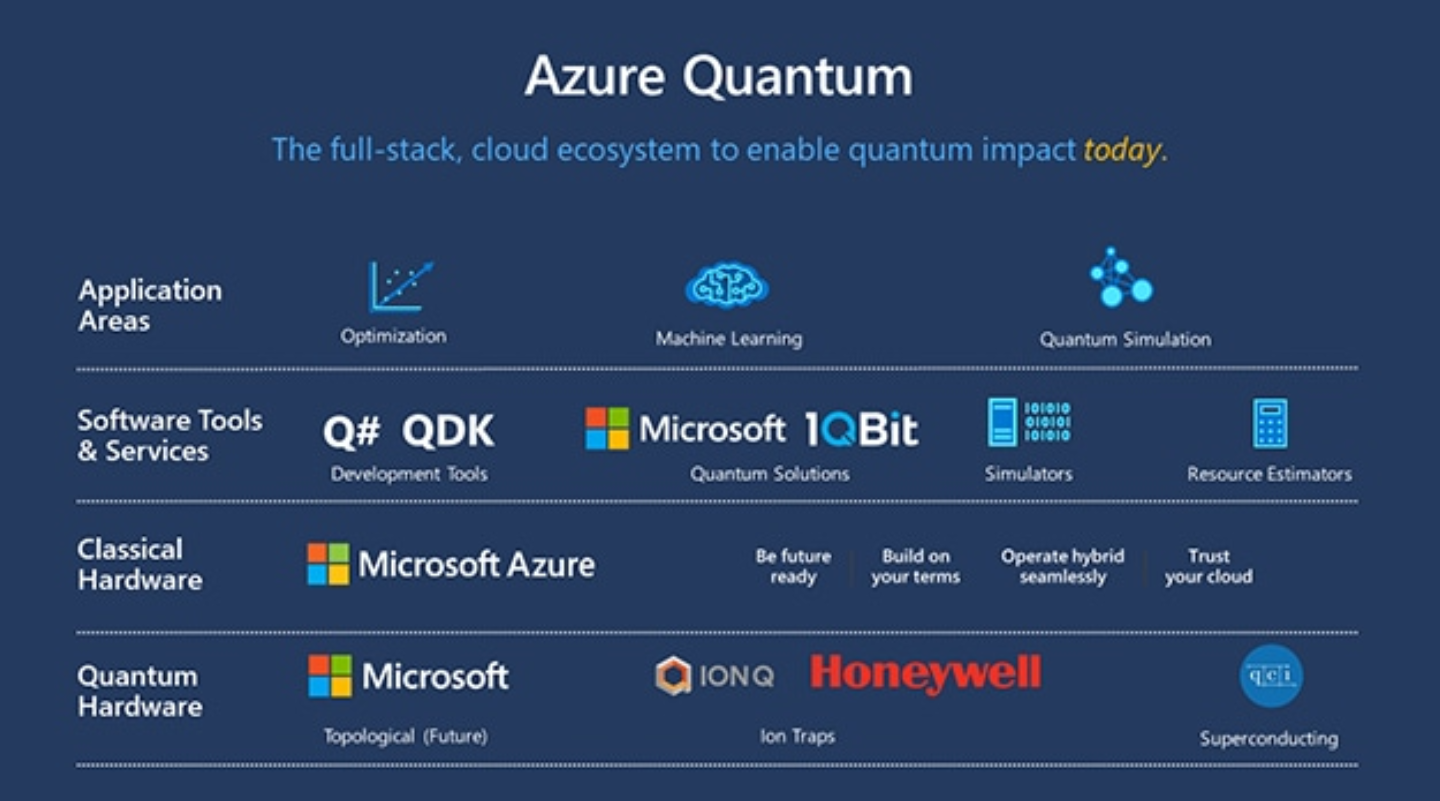
\includegraphics[scale=0.5]{Images/MicrosoftQDKStack.png}
    \caption{Microsoft Azure Quantum Development Stack}
    \label{fig:msQStack}
\end{figure}

\section{Why Microsoft QDK?}
\label{sec:motvQdk}

\begin{itemize}
    \item Microsoft has collaborated with multiple quantum hardware providers to develop quantum solutions. These companies work on different type of technology for realizing a quantum computer such as Ion Traps, Superconducting Qubits and Topological quantum hardware. However, the quantum development kit abstracts the details of underlying hardware and lets the application developers focus on the problem at hand.
    
    \item The Q\# programming language which is part of QDK, is inspired from other high level classical computer programming languages and has a similar syntax for writing programs. This makes learning Q\# easier from traditional high level language programmers.
    
    \item Azure Quantum aims to provide access to quantum hardware for quantum researchers and developers all across the world. This provides an opportunity to quickly validate the functionality of newly developed quantum algorithms and applications on real hardware.
    
    \item Multiple real-world applications are being developed using the the Azure Quantum technology stack which show the usefulness and effectiveness of the development kit as well as quantum computation for real-world problem solving.
    
    \item Microsoft QDK includes a simulator which simulates the working of a real quantum computer on classical hardware. Developers can make use of this feature to run quantum algorithms on classical computer.
    
    \item Microsoft QDK has quantum libraries which are helpful for research in various fields such as Quantum Chemistry, Quantum Machine Learning and Optimization algorithms.
    
    \item All the libraries, Q\# programming language kernel and other resources are open source. This gives an opportunity to developers and researchers to understand the working of a quantum computer as well as contribute to the existing code base.
\end{itemize}

\section{Q\# Programming}
\label{sec:qSharp}
A Q\# program gives a way to interact with qubits and alter the state of those qubits by remaining agnostic about the hardware details of these interactions \cite{cjgronlund_microsoft}. A typical Q\# program consists of \emph{operations} to perform quantum operations, \emph{functions} to perform deterministic classical operations and user defined \emph{types}. Code given below shows an example of a simple operation which creates an array of random numbers using specified number of qubits.

The operation is named GetRandomArray and has a single input parameter named number of built in primitive type Int.  Line 1 also gives the return type of the operation as Int[] - an array of integers. Line 2 assigns the input parameter to local variable named length. The keyword let defines an immutable variable which can not be changed in the later part of the program. Line 3 defines a mutable variable named result of type integer array with length specified by the input parameter. A for loop runs for given number of iterations and creates qubit on line 6 in the zero basis state. Line 8 applies Hadamard gate using the H operation on the qubit to create equal superposition state. The M operation on line 9 measures this qubit to provide a classical result of either One or Zero. This result is then stored in the output array and returned to calling program.

\begin{lstlisting}[caption={Example of Q\# Operation}]
operation GetRandomArray(number : Int) : Int[]{
    let length = number;
    mutable result = new Int[length];

    for (index in 0 .. length - 1) {
        using (qubit = Qubit()) {
            
            H(qubit);
            let measured = M(qubit);
            
            if(measured == One){
                set result w/= index <- 1;
            }
            else{
                set result w/= index <- 0;
            }

            Reset(qubit);
        }
    }
    
    return result;
}
\end{lstlisting}
\BlankLine

Microsoft Quantum Documentation provides detailed information about the features of the Q\# programming language. The quantum program can be called from a host program written in python or any dot net language such as C\#. The full state quantum simulator can be used to execute the quantum subroutine on a classical hardware. Microsoft QDK also provides a resource estimator which gives an estimate of required resources for executing given quantum algorithm.

For learning quantum computing in general with the Q\# language, this documentation also includes code samples known as Quantum Katas. It has implementation examples of basic concepts like quantum superposition and entanglement. Also it includes sample programs for popular quantum algorithms along with their explanations.

%%%%%%%%
\chapter{Design}
\label{sec:desgn}
This chapter discusses the design of the proposed solution. Decision choices of dataset, software frameworks, hardware were made considering the requirements of the research objectives of this dissertation and limitations of current technology. This section explains the reasons and constraints in detail. Additionally, the goal of this design is to produce a software solution which is readily testable on quantum hardware.

\section{Dataset}
\label{sec:dataset}
In machine learning data classification task involves training a model based on given features to predict class of any unknown data sample. Binary classification predicts two separate classes for any given data point while a multi-class classification involves placing data points in more than two classes of labels. This dissertation focuses on binary classification of hand-written images. 

MNIST database \cite{kussul_2004_improved} of hand-written digit images is selected for the research. This database contains images of dimensions 28x28 pixels with grey level value of each pixel specified by a number from 0 to 255. This dataset needs to be pre-processed before using it for data classification. If formatted properly, the developed solution is completely agnostic of the input data dimensions and can work with any kind of database. MNIST database is a well known set of images which can be used for bench-marking the performance of machine learning algorithms for data classification. Figure \ref{fig:mnistEg} shows an example of digits 3 and 6 in the MNIST database.

\begin{figure}[H]
    \begin{subfigure}{0.5\textwidth}
    \begin{center}
    
\includegraphics[width=0.1\linewidth]{Images/mnist_example_digit_3.jpg}
    \end{center}
    \caption{Digit 3}
    \end{subfigure}
    \begin{subfigure}{0.5\textwidth}
    \begin{center}
    
\includegraphics[width=0.1\linewidth]{Images/mnist_example_digit_6.jpg}
    \end{center}
    \caption{Digit 6}
    \end{subfigure}
    \caption{Example images of MNIST Hand-Written Digits}
    \label{fig:mnistEg}
\end{figure}

\section{Solution Architecture}
\label{sec:solArch}

\begin{figure}[H]
    \centering
    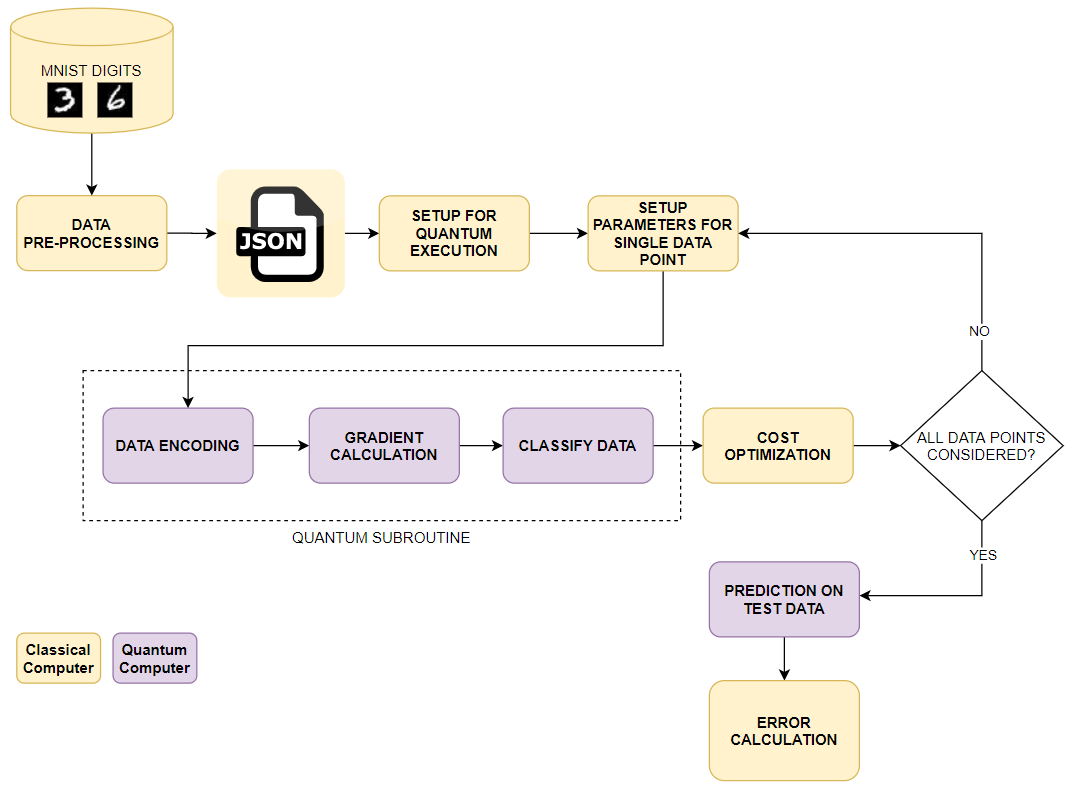
\includegraphics[scale=0.75]{Images/Architecture.png}
    \caption{Solution Architecture and Components}
    \label{fig:solArchComp}
\end{figure}

Figure \ref{fig:solArchComp} shows the design of classical-quantum classifier with all the interacting components. Significance of each individual component is defined in detail further in this section. The architecture involves data exchange between both a classical computer and a quantum computer. Components running on classical computer are shown in yellow boxes while purple boxes show the components executed on a quantum computer.

\subsection{Limitations of Near Term Quantum Computer}
The proposed design is based on the work done by Schuld M. et. al. \cite{schuld_2020_circuitcentric} for developing a data classifier on near term quantum computer. This paper discusses various limitations of currently available quantum computers \cite{perdomoortiz_2018_opportunities} and makes intelligent choices to reduce the impact of these limitations on the performance of the data classifier.

\begin{itemize}
    \item The effective number of qubits is limited in the quantum computers available in the near future. As qubit is the basic building block of quantum information, limited number of qubits put restrictions on the amount of data which can be processed at any given time. IBM's quantum experience provides access to 5 to 15 qubits through the cloud service.
    
    \item Near-term quantum systems are susceptible to environmental interference. Any arbitrary state encoded into a register of qubits available on a quantum computer loses the information due to de-coherence over a period of time.
    
    \item Data encoding, gate operations, measurements and all other stages in quantum computation can result in errors due to electromagnetic interference. These errors can significantly impact accuracy of near-term quantum systems. 
\end{itemize}

Applications developed for the execution on current quantum computers need to take all the aforementioned constraints into consideration.

\subsection{Data pre-processing}
To use the data classifier defined in machine learning library of Microsoft Quantum Development Kit the input data of MNIST images needs to be processed to provide as input. This classical input data is then encoded in quantum computer by the quantum data classifier for further processing. The expected input data format contains values for all the features of training dataset along with corresponding classification labels. This input data also contains values of validation dataset in a similar format. As this is a classical information quantum computers can not process this data directly and a component running on classical computer is required for the conversion. This component involves tasks like loading images into memory, flattening values of pixels in single array, normalization and dimension reduction.

\subsection{Quantum Execution Setup}
This component works as a classical host and is responsible for loading the training and validation data from input file to the objects in memory which are later passed to the quantum subroutine. It acts as an entry point for the application execution. This component also creates an object of the quantum hardware or simulator which is later used for quantum execution. Optionally it is also responsible for defining initial random parameters for the machine learning model. In the current design the component also creates a verbose log file to record all the events during the execution. The host program first selects only the training data samples for learning correlations between different features and with the help of adjustable gate parameters in quantum subroutine creates a model which can map any unknown sample to correct label with high probability. Once the model is ready, the host program inputs validation samples into the quantum program along with values of training parameters and gets the prediction accuracy as output.

\subsection{Quantum Data Encoding}
The classical data generated by the data pre-processing step needs to be converted into quantum representation for processing it in the quantum computer. A basic encoding approach is to map each bit in the classical bytes of information to corresponding qubit value in quantum register. Equation \ref{eq:12} shows the conversion from classical byte to qubit register state.

\begin{equation}\label{eq:12}
    Basic\hspace{3pt}Encoding: 11010101 \Rightarrow \ket{11010101}
\end{equation}

Most quantum computers initialize a qubit in the $\ket{0}$ basis state. Quantum NOT gate or the Pauli-X gate can be applied to convert the $\ket{0}$ state to a $\ket{1}$ state. This method of encoding classical information into quantum computer is easy to implement. However, it is not efficient due to its requirement of higher number of qubits. A 32-bit integer value in classical information will require corresponding 32 qubits. Publicly available quantum computers currently provide access to around 10-15 qubits making Basic Encoding unsuitable for near-term qunatum applications.

Many quantum algorithms including the data classifier in Microsoft QDK use amplitudes of an arbitrary state of a qubit to encode classical information \cite{schuld_2020_circuitcentric}. This method is referred to as Amplitude Encoding. The data encoding component is a part of data classifier library which takes the classical data as input and using the state preparation circuit initializes amplitudes of a string of qubits to represent equivalent quantum information. An arbitrary state of qubit is represented in terms of phase as given below. The amplitudes of the qubit are expressed in terms of phase $\theta$.

\begin{equation}\label{eq:13}
    \ket{\psi} = cos\hspace{2}\dfrac{\theta}{2}\hspace{2}\ket{0} + e^i^\varphi \hspace{2}sin\hspace{2}\dfrac{\theta}{2}\hspace{2}\ket{1}
\end{equation}

Quantum rotation gate can prepare any arbitrary state by taking the rotation angle as input. The state preparation circuit adjusts rotation parameter $\theta$ of combination of rotation gates to generate any arbitrary state using the values of input feature vector X = \{$x_1, x_2, x_3, ....., x_n$\}. As shown in table  \ref{tab:sampleImages}, we are given a set of 4 images. Each image has values for its 4 individual pixels and corresponding classification label. Consider the first image having 4 pixel values as 15, 44, 134 and 207. To encode these 4 values we need 4 amplitudes which can be represented by a 2 qubit register. The state of a 2 qubit register can be given by \(\ket{\psi}=\alpha\ket{00} + \beta\ket{01} + \gamma\ket{10} + \delta\ket{11}\) where \(\alpha\), \(\beta\), \(\gamma\), \(\delta\) are the amplitudes of the basis states and \(\alpha^2 + \beta^2 + \gamma^2 + \delta^2 = 1\). We can normalize the feature vector by dividing each value by the total sum. Here the sum = 15 + 44 + 134 + 207 = 400. Dividing each feature value by 400 gives us squares of amplitudes of the 2-qubit state vector. Hence amplitude values can be specified by \(\alpha^2\) = 0.0375, \(\beta^2\) = 0.11, \(\gamma^2\) = 0.335 and \(\delta^2\) = 0.5175. By adjusting parameters of a 2x2 unitary gate in the state preparation circuit the 2-qubit arbitrary state can be prepared with the required amplitude values.

\begin{table}[H]
\begin{center}
\begin{tabular}{|c|c|c|c|c|c|}
\hline
\textbf{Sample No.} & \textbf{Pixel 1} & \textbf{Pixel 2} & \textbf{Pixel 3} & \textbf{Pixel 4} & \textbf{Label} \\
\hline
1 & 15 & 44 & 134 & 207 & 1\\
\hline
2 & 54 & 25 & 183 & 190 & 1\\
\hline
3 & 114 & 230 & 1 & 89 & 0\\
\hline
4 & 87 & 5 & 187 & 254 & 1\\
\hline
\end{tabular}
\end{center}
\caption{4 images of 4 pixels each} 
\label{tab:sampleImages}
\end{table}

The state preparation circuit requires the count of values N, in the feature vector to be an exact power of 2. In a real world dataset this is achieved by choosing padding such that \(N^'\) = N + D and \(N^'\) is some exact power of 2 \cite{schuld_2020_circuitcentric}. This is similar to having more nodes in the first hidden layer of a neural network than the previous layer. Amplitude encoding method requires poly-logarithmic quantum resources with respect to the input sample size and is suitable for near-term quantum hardware. The state preparation circuit can be thought of as a black box which encodes the input feature vector into amplitudes of quantum state as shown in figure .

\begin{figure}[H]
    \centering
    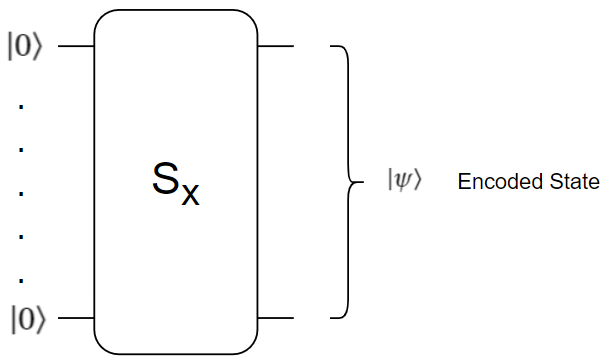
\includegraphics[scale=0.6]{Images/StatePreparationCircuit.PNG}
    \caption{State Preparation Circuit}
    \label{fig:statePrepCirc}
\end{figure}

\subsection{Gradient Calculation}
Classical machine learning algorithms depend on gradient descent calculation \cite{bottou_2010_largescale} for reducing the error in predictions and incremental learning. Each feature is associated with its corresponding parameter which decides the weight of the feature in prediction of labels. Gradient descent algorithm takes partial derivatives of the cost function with respect to each individual parameter to update the parameters gradually with specified learning rate to minimize prediction error. Cost optimization algorithms converge to an optimum value beyond which there is no significant improvement is achieved in the prediction error by applying the gradient descent calculation. Parameter vector learned by this method is then used for prediction of labels on unknown data with same features.

Similar to the classical machine learning method, the classification algorithm in quantum development kit uses gradient descent calculations \cite{schuld_2020_circuitcentric} to incrementally learn parameters for data classification. The n qubit register is prepared in a quantum state by the state preparation circuit to represent the input feature vector. The gradient calculation circuit takes this encoded state \(\ket{\psi}\) of n qubits as input and maps it to another quantum state \(\ket{\psi}^'\) such that \(\ket{\psi}^'\) = \(U_\theta \ket{\psi}\). Here \(U_\theta\) represents an unitary operation which can be decomposed into individual logical quantum gates and implemented on a quantum hardware.

\begin{figure}[H]
    \centering
    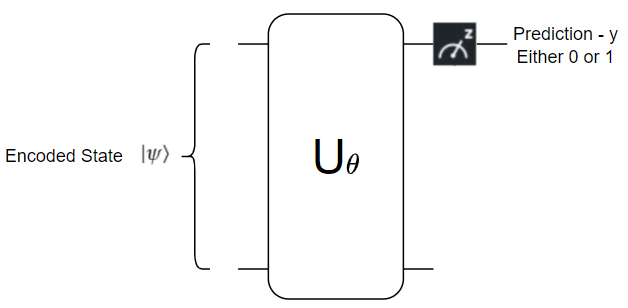
\includegraphics[scale=0.9]{Images/GradientCalculationCircuit.PNG}
    \caption{Gradient Calculation Circuit}
    \label{fig:gradeCalcCirc}
\end{figure}

The unitary circuit \(U_\theta\) can be broken down into individual quantum gates. This circuit typically comprise of single qubit and two qubit controlled gates. A single qubit quantum gate can be represented in terms of angle as given by equation \ref{eq:14} \cite{schuld_2020_circuitcentric}. Here \(\phi\) represents a global phase and can be ignored. This gives three parameters \(\alpha\), \(\beta\) and \(\gamma\) per quantum gate which can be learned. These parameters can be translated to physical control parameters such as the intensity of the laser on a quantum hardware.

\begin{equation}\label{eq:14}
G(\alpha, \beta, \gamma, \phi) = e^{i\phi}
\begin{bmatrix}
e^{i\beta}\hspace{2pt}cos\hspace{2pt}\alpha & e^{i\gamma}\hspace{2pt}sin\hspace{2pt}\alpha\\
-e^{-i\gamma}\hspace{2pt}sin\hspace{2pt}\alpha & e^{-i\beta}\hspace{2pt}cos\hspace{2pt}\alpha
\end{bmatrix}
\end{equation}

Similarly a 2-qubit controlled gate can be represented by the matrix given in the equation \ref{eq:15}. This representation shows that even 2-qubit gates have 3 learnable parameters \(\alpha\), \(\beta\) and \(\gamma\). These multi qubit gates are useful to break the symmetry of dependency between variables introduced by the single qubit gates. 

\begin{equation}\label{eq:15}
C_1(G_0) = \begin{bmatrix}
1 & 0 & 0 & 0\\
0 & e^{i\beta}\hspace{2pt}cos\hspace{2pt}\alpha & 0 & e^{i\gamma}\hspace{2pt}sin\hspace{2pt}\alpha\\
0 & 0 & 1 & 0\\
0 & -e^{-i\gamma}\hspace{2pt}sin\hspace{2pt}\alpha & 0 & e^{-i\beta}\hspace{2pt}cos\hspace{2pt}\alpha
\end{bmatrix}
\end{equation}

Figure \ref{fig:gateBlocks} shows blocks of different entangling layers of gates in a quantum classifier working on a 8-qubit register. The given circuit contains total 33 gates each with 3 controllable parameters. Microsoft quantum development kit currently provides 3 different type of controlled rotation layers namely LocalRotationsLayer, PartialRotationsLayer and CyclicEntanglingLayer. Various combinations of these layers can be added to the classifier architecture to achieve desired results in data classification tasks. This architecture model of data classifier provides various control parameters which can be varied to improve the performance. These control parameters include factors such as number of layers in the architecture, number of qubits acted on by given layer, rotation axis and range of connection between qubits. In the circuit shown below, range of conncetion is 1 for the layer B1 and 3 for the layer B3.  Other controllable hyper-parameters are learning rate, number of epochs, batch size of input feature vector and number of measurements of the prediction qubit.

\begin{figure}[H]
    \centering
    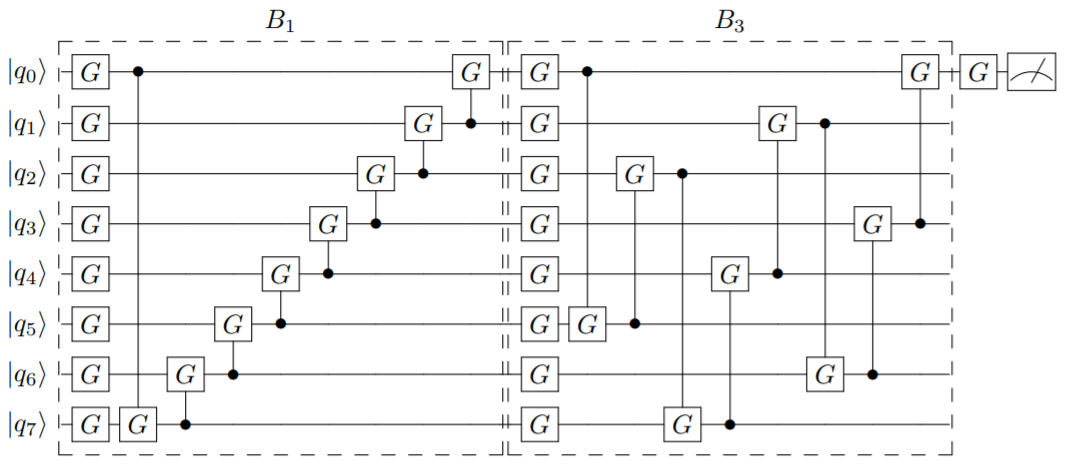
\includegraphics[scale=0.7]{Images/GradientGateBlocks.PNG}
    \caption{Layers of gate combinations in Quantum Classifier \cite{schuld_2020_circuitcentric}}
    \label{fig:gateBlocks}
\end{figure}

The cost function of the prediction algorithm is given by equation \ref{eq:16} where training set is D = ${(x^1, y^1),....(x^M, y^M)}$.

\begin{equation}\label{eq:16}
C(\theta, b; D) = \sum_{m=1}^{M} |\pi(x^m; \theta, b) - y^m|^2
\end{equation}

where \(\theta\) is the parameter configuration and b is the bias. The function $\pi$ gives the probability of measuring qubit \(q_0\) in the state 1 for given parameters.

\subsection{Measurement and Cost Optimization}
The measurement of the qubit $q_0$ from the model circuit $U_\theta$ provides the prediction value for given set of features. Bias b is added for producing continuous output. The model prediction function is given by the equation \ref{eq:17} \cite{schuld_2020_circuitcentric}.

\begin{equation}\label{eq:17}
    f(x)= 
\begin{cases}
    1,& \text{if } \pi(x; \theta) > 0.5\\
    0,              & \text{otherwise}
\end{cases}
\end{equation}

As the measurement output is probabilistic, the entire circuit operation is repeated multiple times for determining the probability of measuring qubit $q_0$ in state 1. Depending on the expected outcome for given sample in the training data, gate parameters are altered to achieve desired measurement with high probability. These measurements are repeated for all the training samples and a parameter configuration is found which produces lowest error on the training data.

\subsection{Test Data Validation}
The model circuit learned in the previous steps produces a set of parameters for given architecture of gates in different layers of quantum gates. Using these parameters and the features in the validation data, predictions can be obtained. These predictions can then be used to evaluate accuracy of given circuit architecture.

Next section discusses the implementation details based on the proposed design of the quantum classification system.

%%%%%%%%
\chapter{Implementation}
\label{sec:impl}
The implementation of the classification program consisted of selecting and pre-processing the dataset and evaluating the performance of QDK classifier on the selected dataset. Multiple iterations were performed to gather as much data as possible for the assessment of the performance.  

\section{Data Processing}
\label{sec:dataprocess}
This dissertation uses MNIST images of handwritten digits. This dataset is divided into training images and test images. It consists of 60000 training images and 10000 test images \cite{kussul_2004_improved}. Multiple classical machine learning algorithms use this data to train classifier model and check the accuracy on validation images.

\begin{figure}[H]
    \centering
    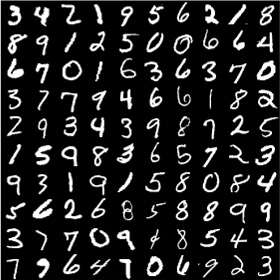
\includegraphics{Images/MnistExamples.jpg}
    \caption{Example of MNIST Handwritten digits}
    \label{fig:mnistEg}
\end{figure}

Some neural networks have been able to achieve human equivalent accuracy on this data. As the adoption for this dataset is very high among multiple classical machine learning algorithms, it became a natural choice for experimenting the implementation of quantum classifier on MNIST data. This database also gives an opportunity to showcase one of the methods of encoding classical image data into quantum computer. Figure \ref{fig:mnistEg} shows example of some of the images from the MNIST database. 

Each of the MNIST image consists of 28x28 pixel dimensions totalling to 784 pixels per image. Every pixel in the image is represented by a value from 0 to 255. This value gives the grey level of each of these pixels. This gives rise to 784 features to be processed for learning the model for classification. Due to few challenges discussed in the later part of the dissertation, it was not feasible to use the entire dataset for processing using the quantum subroutine. Experiments were carried out using 100 to 2000 training images from the database while validating the model accuracy on 20-200 test images. Furthermore, only a few experiments were performed using the entire set of 784 features. For most of the iterations, the number of learnable parameters were reduced by using the dimensionality reduction algorithm known as Principal Component Analysis (PCA). First set of images for data classification contains hand-written images of the digits 3 and 6 having very low resemblance among each other while other set contains images of the digits 1 and 7 with higher resemblance. This selection was intentional to compare the accuracy of the quantum classifier on different sets of images.

\subsection{Dimensionality Reduction using Principal Component Analysis (PCA)}
The algorithm Principal Component Analysis or PCA \cite{firmin_2019_tidying} is used to find most important independent features in a multi-dimensional dataset which capture the highest variation in the dataset. It takes advantage of the existence of the co-variance between different features of a sample to represent the given sample with less number of features but with highest possible resemblance with the original sample. 

\begin{figure}[H]
    \centering
    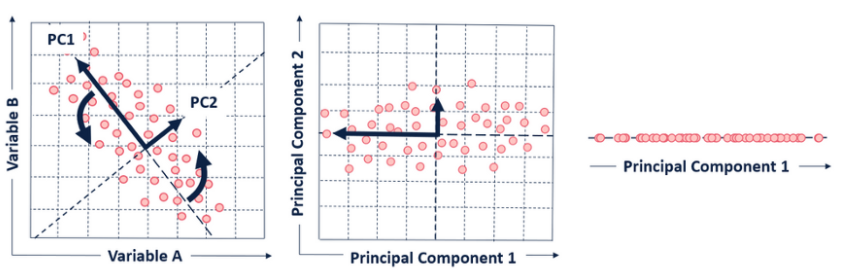
\includegraphics{Images/PCA.PNG}
    \caption{Principal Components of 2 feature dataset}
    \label{fig:pca}
\end{figure}

This algorithm provides a way to approximate higher dimensional data with lower number of dimensions thus achieving dimensionality reduction \cite{gorban_2007_principal}. First principal component gives the highest amount of variance in the given dataset. Second highest variance is represented by the principal component 2 and so on. Principal components are represented by the eigenvalues and eigenvectors which represent the scale and direction of variation among the features. A simple example of the principal components capturing variance between two variables is shown in figure \ref{fig:pca}. A quantum algorithm for the principal component analysis of a dataset is already developed \cite{lloyd_2014_quantum}. However, this dissertation makes use of SKLEARN's python library on classical computer to perform PCA on the selected MNIST dataset. Experiments were performed by selecting 2 to 30 principal components from the available 784 features of each MNIST image. The python script loads all the training and test images in memory and applies the PCA algorithm from existing library to produce a JSON file. This file is then consumed by the classification algorithm.

\begin{algorithm}
	\SetAlgoLined
	 $imageQueue \gets imageFiles$\;
	 $numOfPrincipalComponents \gets 30$\;
	 $normalizationFactor \gets 250$\;
	\While{imageQueue is not empty}{
		image = imageQueue.pop()\;
		label = image.label\;
		
		flattenedImage = image.flatten()\;
		
		components = sklearn.PCA(flattenedImage)\;
		reducedComponents = reduce(components, numOfPrincipalComponents)\;
		
		normalized = normalizeValues(reducedComponents, normalizationFactor)\;
		
		dumpToJson(components, label)\;
	}
	\caption{Data Pre-Processing}
	\label{algo:1}
\end{algorithm}

The output JSON file is divided into two sections each for the training and testing dataset. Additionally, each section has feature vector values with floating-point precision of 3 and another vector for corresponding labels. 

\section{Data Classification using QDK}
\label{sec:qClassifier}

\subsection{Training}

Quantum programs written in Q\# can be called as a subroutine from python or dot net languages such as C\#. The classical host program for this dissertation is written in C\#. This program reads the JSON file and builds objects of training data and validation data which can later be utilized by quantum functions. The Dataset object contains two fields for holding Lists of training data and validation data. Both these lists are further divided into list of features and labels. Some of the code for the implementation of this quantum classifier is taken from samples provided by Microsoft quantum development community \cite{mykhailova_2020_microsoftquantumkatas, granade_2020_microsoftquantum}.

\begin{lstlisting}[caption={C\# Data Objects}]
class LabeledData
{
    public List<double[]> Features { get; set; }
    public List<long> Labels { get; set; }
}

class DataSet
{
    public LabeledData TrainingData { get; set; }
    public LabeledData ValidationData { get; set; }
}
\end{lstlisting}

Once these objects are loaded with data from JSON file, a Q\# subroutine is called for training model circuit by passing both the training features and labels. The operation TrainMnistModel in Q\# program builds a ClassifierStructure by combining different layers of ControlledRotation layers. For the implementation of this dissertation multiple combinations of LocalRotationsLayer, PartialRotationsLayer and CyclicEntanglingLayer were used while building the ClassifierStructure. Various controllable parameters such as the rotation axis, number of qubits the gates act on and range of qubit connections were altered for each execution to compare performance. Input training data is converted into an array of type LabeledSample, defined in QDK library. It encapsulates each input sample with its class label in an object. Depending on the dimensions of input features, a random set of initial training parameters are generated using the Microsoft.Quantum.Math.RandomReal operation. This operation generates random double values. The SamplingSchedule class is used to fetch batches from training and validation set of samples. The function DefaultTrainingOptions defined in Microsoft.Quantum.MachineLearning is used to specify various hyper-parameters such as learning rate, NMeasurements and number of epochs. For this dissertation, learning rate was kept constant at 0.4 for most executions while the number of epochs were 2 to 4. The NMeasurements were 10000 for most of the experiments. Multiple iterations of the program execution are required to understand the impact of these hyper-parameters on the accuracy of the classifier.

The operation TrainSequentialClassifier takes the Classifier architecture as input along with the array of LabeledSample which contains input features. The SamplingSchedule dictates the classifier to select batch of samples for training and validation. This operation outputs the parameters of given classifier along with the bias between the classes. These parameters and bias can later be used for prediction on validation dataset.

\subsection{Validation}
The machine learning library in Microsoft QDK provides an operation  ValidateSequentialClassifier for testing model cicuit on the test data. It takes the same classifier architecture used while training as input with the circuit parameters and gate as input. The function runs the model circuit on validation data to calculate classification misses. It returns the result as an object of type ValidationResults which only contains the information about number of misclassifications and number of samples. To dive deeper into the actual predictions made by the operation, the code was taken from the open source library of QDK and used for analysis. This data of predicted labels can be compared with actual labels to visualize the boundary of classified labels.

\section{Data Classification using Classical Libraries}
\label{sec:classicalDataClass}
\begin{figure}[H]
    \centering
    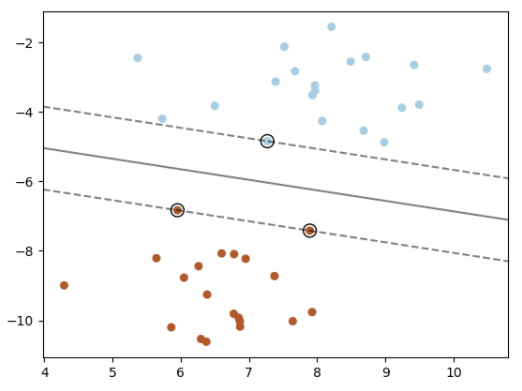
\includegraphics{Images/SVMHyperplane.PNG}
    \caption{Example of SVM Data Classification with 2-dimensional dataset}
    \label{fig:svmHypPlane}
\end{figure}

MNIST is a very common database for evaluating machine learning algorithms for data classification and multiple results are already available for bench-marking the performance. However, in this dissertation, a classical classifier was executed on the same dataset used for quantum data classification. While comparing the results of these experiments one needs to be aware of the fact that all the quantum executions were performed using quantum simulator provided by Microsoft QDK.

The classical classifier is based on SKLEARN's SVM library \cite{pedregosa_2011_scikitlearn} which uses the Support Vector Machine algorithm for data classification. SVM algorithms are supervised machine learning algorithms for data classification and few other machine learning applications. It divides the classes of a multi-dimensional dataset by using a hyper-plane that maximizes the margin with the data of both the classes \cite{smola_2004_a}. Using this hyperplane the algorithm then makes the predictions on actual validation data. Figure \ref{fig:svmHypPlane} shows an example of separating line for a 2-dimensional dataset.

The implementation of classical classifier includes reading the JSON file to create objects with the training and validation data. This data is then provided for training to the SVC function with minimal input parameters. Once the model is trained it is validated on the test data to calculate accuracy of the algorithm. This algorithm is capable of handling all 784 features of the input MNIST images. However, for fair comparison of both the computing paradigms, classical classifier was executed on dataset with 10-30 features which are obtained by the PCA dimensionality reduction algorithm.

%%%%%%%%
\chapter{Results}
\label{sec:resEval}
This chapter discusses results obtained after multiple iterations of experiments with the quantum data classifier provided by Microsoft QDK. Due to unavailability of quantum hardware all the experiments were performed on a quantum simulator running on a classical machine (Laptop). 

\begin{figure}[H]
    \centering
    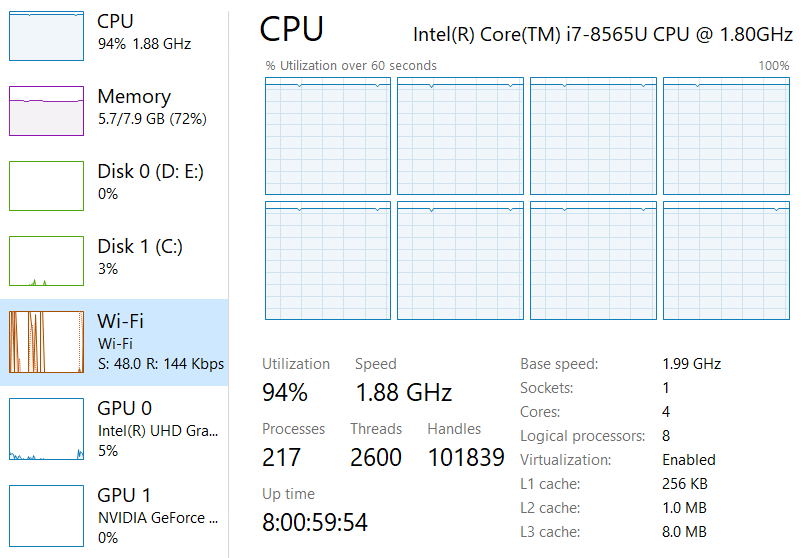
\includegraphics[scale=0.9]{Images/CPUandMemoryUtilization2.PNG}
    \caption{Computer Configuration and CPU Utilization}
    \label{fig:cpuConfig}
\end{figure}

The laptop used for executions, had 8 gigabytes of Random Access Memory and was equipped with Intel Core i7-8565U processor clocked at a frequency of 1.8GHz. The processor has a base speed of 1.99 GHz with L1 cache of 256 KB. It also has 8 logical processors capable of executing threads simultaneously. Figure \ref{fig:cpuConfig} shows the configuration of used machine in detail. Also it shows the CPU and memory utilization during the execution of the quantum circuit training. The program runs under the name of QDK.exe and figure \ref{fig:cpu} shows the CPU and memory utilization specific to this process.

\begin{figure}[H]
    \centering
    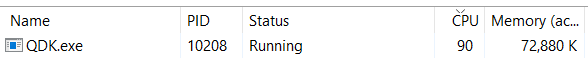
\includegraphics{Images/CPUandMemoryUtilization.PNG}
    \caption{CPU and Memory Utilization}
    \label{fig:cpu}
\end{figure}

Figure \ref{fig:compareResult} shows a comparison between results obtained by using quantum classifier and classical SVM classifier. These results are obtained after training model on 2000 images of digits 3 and 6 and testing the model on 200 images of digits 3 and 6. Only 10 principal components were used for this execution. In the plot shown in figure \ref{fig:compareResult}, first and second principal components are plotted. The z axis shows the digit the points belong to. Points are color coded based on the accuracy of prediction. Yellow points show incorrect results obtained from the trained model, while blue points display correctly predicted images.

\begin{figure}[H]
    \begin{subfigure}{0.5\textwidth}
    \begin{center}
    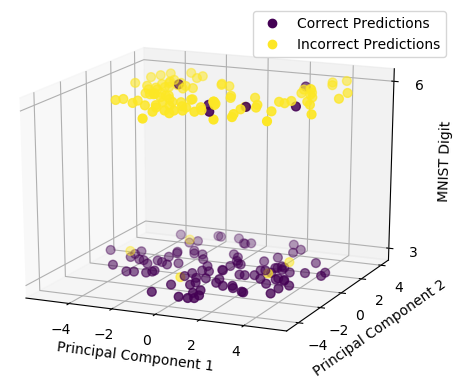
\includegraphics[width=1.0\linewidth]{Images/QuantumPredictions.PNG}
    \end{center}
    \caption{Classification using Quantum Classifier}
    \end{subfigure}
    \begin{subfigure}{0.5\textwidth}
    \begin{center}
    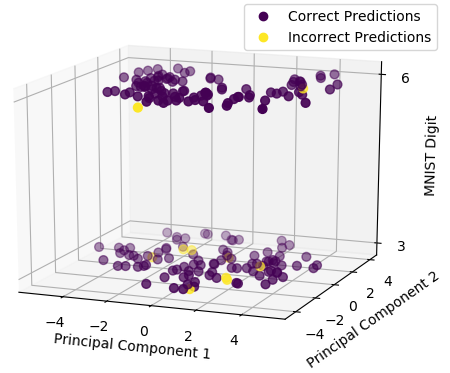
\includegraphics[width=1.0\linewidth]{Images/ClassicalPredictions.PNG}
    \end{center}
    \caption{Classification using Classical (SVM) Classifier}
    \end{subfigure}
    \caption{Comparison of Quantum and Classical executions}
    \label{fig:compareResult}
\end{figure}

Multiple such iterations were executed on quantum simulator by selecting subset of the MNIST database. All the experiments were completed only for the digits 3 and 6 due to time constraints. Table \ref{tab:results} shows results obtained for a few of the executions out of the total 13 experiments performed. It lists down number of features used for training and validation per image. Classifier architecture is also specified in the table. Learning rate and number of epochs were kept constant for most of the experiments to isolate the effect of classifier structure on the accuracy of model circuit. The runtime of each of these experiments is also shown in the table. Detailed logs are captured during each of these executions which show the steps in training and validation of the data classification.

\begin{table}[H]
\begin{center}
\resizebox{\textwidth}{!}{
\begin{tabular}{|c|c|c|c|c|c|c|}
\hline
\textbf{\makecell{Number \\ of Features}} & \textbf{\makecell{Number \\ of Images}} & \textbf{Layers} & \textbf{\makecell{Learning \\ Rate/Epochs}} & \textbf{Result} & \textbf{Execution Time} & \textbf{Accuracy}\\
\hline
2 & \makecell{Train - 100 \\ Test - 20} & \makecell{2 LocalRotationsLayer \\ 1 CyclicEntanglingLayer \\ 1 PartialRotationsLayer} & 0.4/4 & Passed & 2 hours & 43\% \\
\hline
10 & \makecell{Train - 195 \\ Test - 28} & \makecell{2 LocalRotationsLayer \\ 1 CyclicEntanglingLayer \\ 1 PartialRotationsLayer} & 0.4/4 & Passed & 2 hours & 60\% \\
\hline
784 & \makecell{Train - 195 \\ Test - 28} & \makecell{1 LocalRotationsLayer} & 0.4/4 & \makecell{Failed \\ IDE Crash} & 14 Days & NA \\
\hline
30 & \makecell{Train - 2000 \\ Test - 200} & \makecell{2 LocalRotationsLayer \\ 1 PartialRotationsLayer} & 0.4/2 & Passed & 6 Days & 55\% \\
\hline
30 & \makecell{Train - 2000 \\ Test - 200} & \makecell{2 LocalRotationsLayer \\ 1 CyclicEntanglingLayer} & 0.4/2 & Passed & 6 Days & 55\% \\
\hline
10 & \makecell{Train - 2000 \\ Test - 200} & \makecell{1 LocalRotationsLayer \\ 2 CyclicEntanglingLayer} & 0.4/2 & Passed & 3 Days & 50\% \\
\hline
\end{tabular}
}
\end{center}
\caption{Results for few experiments using Microsoft QDK Quantum Data Classifier on a Quantum Simulator} 
\label{tab:results}
\end{table}

For comparing the accuracy of quantum executions with classical algorithms, experiments were performed on the same dataset with SKLEARN's implementation of multiple classification algorithms. 

\begin{table}[H]
\begin{center}
\begin{tabular}{|c|c|c|c|}
\hline
\textbf{\makecell{Number \\ of Features}} & \textbf{\makecell{Number \\ of Images}} & \textbf{Algorithm} & \textbf{Accuracy}\\
\hline
10 & \makecell{Train - 2000 \\ Test - 200} & \makecell{SVM} & 95\% \\
\hline
10 & \makecell{Train - 2000 \\ Test - 200} & \makecell{Logistic Regression} & 40\% \\
\hline
10 & \makecell{Train - 2000 \\ Test - 200} & \makecell{Gaussian Process Classifier} & 91.5\% \\
\hline
10 & \makecell{Train - 2000 \\ Test - 200} & \makecell{K Neighbors Classifier} & 92.5\% \\
\hline
\end{tabular}
\end{center}
\caption{Results of SKLEARN's Classical Classifiers on selected MNIST images} 
\label{tab:resultsClassical}
\end{table}

Table \ref{tab:resultsClassical} shows results obtained after execution of classical libraries on a dataset of 2000 training images with 10 principal components. Test dataset contained 200 images. These experiments used default settings of the classical algorithms and the hyper-parameters were not changed manually. All the classical executions only took few seconds of execution time on the same classical machine used by quantum simulator. 

%%%%%%%%%%%%%%%%%%%%%%%%%%%%%%%%%%%%
\chapter{Discussion}
\label{sec:discus}
This section discusses the results obtained in the experiments. Also, it lists down all the challenges faced which influenced few of the decisions taken while performing the research. Following observations can be derived from the results.

\begin{itemize}
    \item As the experiments were performed on a quantum simulator rather than actual quantum hardware, execution time for each experiment was unreasonably high. Selecting smaller datasets can reduce this time. However, performance on smaller datasets does not represent the actual accuracy of the algorithms on real-world dataset.
    
    \item Almost all of the classical algorithms achieved more than 90\% accuracy on the same dataset with 10 features per image while the maximum accuracy achieved by the quantum algorithm in the experiments is 55\% with 30 features of 2000 training images and 200 test images.
    
    \item There are a lot of misclassifications for the image of digit 6 as compared to digit 3 images. 
    
    \item Execution time of classical algorithms is only a few seconds which is exponentially better than the performance of quantum simulator.
    
    \item With the Intel Core i7-8565U processor clocked at a frequency of 1.8GHz, the CPU utilization remained at 90\% or more for entire execution time of quantum simulator. Memory footprint of around 73MB is reasonable.
    
    \item This execution time for binary classification task, suggests an exponential time requirement for multi-class classification experiment, which can be performed by extending the binary classification algorithm with one versus all strategy \cite{schuld_2020_circuitcentric}.
    
    \item Due to unavailability of a real quantum hardware, all the experiments were performed on a quantum simulator running on a classical computer. This restricts us to make any claim about the quantum superiority or inferiority over classical computers.
\end{itemize}

\section{Challenges}
\begin{itemize}
    \item This research expected the access to Azure Quantum to be available during the implementation phase. However, it is not available for public use till the writing of this dissertation. 
    This became a challenge to validate the superiority of quantum computer.
    
    \item Only a single classical computer was used throughout the implementation phase. For parallel experiments, few other options such as using cloud virtual machines or remotely accessing laboratory computers were considered. However, these computer either did not meet the required capacity for the experiments or did not provide required access permissions.
    
    \item Microsoft's quantum development kit is still evolving. The current APIs defined in machine learning library do not have comprehensive documentation to understand inner working of the algorithms. A request was raised for adding details to the available documentation with the development team.
    
    \item It is important to perform as many experiments as possible with the available technology by changing various parameters of the algorithm to understand the capabilities. The exponential increase in execution time on quantum simulators restricted this research to perform a lot of experiments. This might not be a challenge on a real quantum hardware.
    
\end{itemize}

%%%%%%%%%%%%%%%%%%%%%%%%%%%%%%%%%%%%
\chapter{Conclusion}
\label{sec:concl}
With the quantum supremacy in sight, there is a lot of hope from quantum computing field to solve few of the intractable problems for current classical computers. This research was able to provide a glimpse of the capabilities and current challenges of quantum computing. This research was able to achieve the first objective of learning about quantum computation and quantum information processing. This knowledge is useful for the readers who are absolute beginners in this research domain. Applications of quantum computers are beyond the single area of machine learning. A real quantum hardware has started being available through cloud computing which can give a chance to perform the experiments on exponentially faster hardware for quantum calculations.

The limited number of experiments performed during this research do not show any advantage of the quantum simulators on classical algorithms for data classification tasks. Highest data classification accuracy of around 55\% after 6 days of execution is not exciting given the comparison with the performance of classical computers. However, altering the classifier architecture and few other parameters with faster execution on a quantum hardware might show improvements over the achieved results. 

This research has been able to provide an end to end implementation of a hybrid application for image classification of MNIST database. The code base of this application is a combination of multiple available samples and online articles \cite{mykhailova_2020_microsoftquantumkatas, granade_2020_microsoftquantum}. The hybrid application can be used as a starting point for further research. Additionally, the application involves C\# to Q\# data transfer samples which can be used for building more complex applications.

\section{Future Work}
As discussed in the challenges section this research had multiple limitations while performing the experiments. There is a lot of scope for further improvements and research in the same domain. This section suggests possible directions of future research in quantum application development.

\begin{itemize}
    \item The quantum subroutine used for training and validation of classification algorithm can be executed on a real quantum hardware to measure the performance. This will provide an opportunity to identify bottlenecks in the performance of quantum classifier algorithm.
    
    \item Although the research was done on MNIST images, further research can involve much richer databases for data classification. These datasets can be selected with an intention to compare quantum algorithms with benchmark results of classical machine learning algorithms.
    
    \item Microsoft's QDK is only one of the multiple quantum development frameworks available currently for the use by developer community. Similar experiments can be performed on quantum environments provided by IBM's QISKIT, Google's Cirq, Amazon's BRAKET and few other vendors.
    
    \item This research was based on Circuit-Centric Quantum Classifier \cite{schuld_2020_circuitcentric} algorithm which is mainly targetted for near-term quantum hardware. Once the quantum systems evolve, further research can be focused on implementing other quantum machine learning algorithms on the same datasets and the performance of these algorithms can be compared both in terms of execution time and accuracy.
    
    \item Further research in the field of performance improvement of quantum simulators can help developers to test solutions faster.
\end{itemize}

%%%%%%%%%%%%%%%%%%%%%%%%%%%%%%%%%%%%
\nocite{}
\bibliographystyle{plain}
\bibliography{ReferenceList}

\appendix
\chapter{Appendix}

\begin{lstlisting}[caption={Sample JSON Input file for Data Classification}]
{
  "TrainingData": {
    "Features": [
        [x1.1, x1.2, x1.3], [x2.1, x2.2, x2.3], ..., ...
    ],
    "Labels": [
        y1, y2, ..., ...
    ]
  },
  "ValidationData": {
    "Features": [
        [x1.1, x1.2, x1.3], [x2.1, x2.2, x2.3], ..., ...
    ],
    "Labels": [
        y1, y2, ..., ...
    ]
  }
}
\end{lstlisting}

\begin{itemize}
    \item Code and execution logs available at: \url{https://github.com/J1990/QuantumExperiments}
    
    \item 3Blue1Brown \cite{a3blue1brown_2016_vectors} is a very nice YouTube channel created by Grant Sanderson for building intuition regarding linear algebra and other mathematical concepts.
    
    \item Code of Microsoft Quantum Libraries: \url{https://github.com/microsoft/QuantumLibraries}
    
    \item An issue was raised to add circuit images of the model circuit in the component used for quantum gradient calculation for better understanding of the internal details. Issue Link: \url{https://github.com/microsoft/QuantumLibraries/issues/300}.
    The development team came back with a response to this issue as below. This can be added in further research.
    
    \begin{displayquote}
    \emph{Thanks for raising this, @J1990! We'll look at how to add more examples of using those QML library functions in API documentation. As a side note, you may also be interested in the feature at:} \url{https://github.com/microsoft/iqsharp/pull/231}
    \end{displayquote}
\end{itemize}
\end{document}